\section{Week 7: 2nd - 8th March 2026}

\subsection{Monday 2nd March}

\begin{itemize}
    \item Today, I implemented some different optimisation routines that I read about over the weekend. I had some success and some failures.
    \item I tried to use a global optimiser such as "scipy.differential\_evolution" but it essentially gave the same results as the Nelder-Mead method.
    \item I tried to use GPy, like it the main GPR paper, but I think it was out of my understanding and I didn't really understand how to get it to work properly. It did not give good results at all. I will not show my results here.
    \item I tried to use MCMC and I got kind of reasonable results.
    \begin{itemize}
        \item I did MCMC with two cases, one fitting with a spectral index and another time without the spectral index. Both results are shown below
        \item It can be seen that with the case without the spectral index, the parameters are better constrained, especially with the foreground parameters. 
        \item In the case with the spectral index, the parameters hit the upper bounds and are not well constrained at all.
    \end{itemize}

\end{itemize}

\clearpage

\subsubsection{MCMC with spectral index}

\begin{figure}[hbt!]
    \centering
    \includegraphics[width=1\linewidth]{outputs/week8/mcmc_chain_with_sp_indx_fg_1.pdf}
    \caption{Enter Caption}
    \label{fig:placeholder}
\end{figure}

\begin{figure}[hbt!]
    \centering
    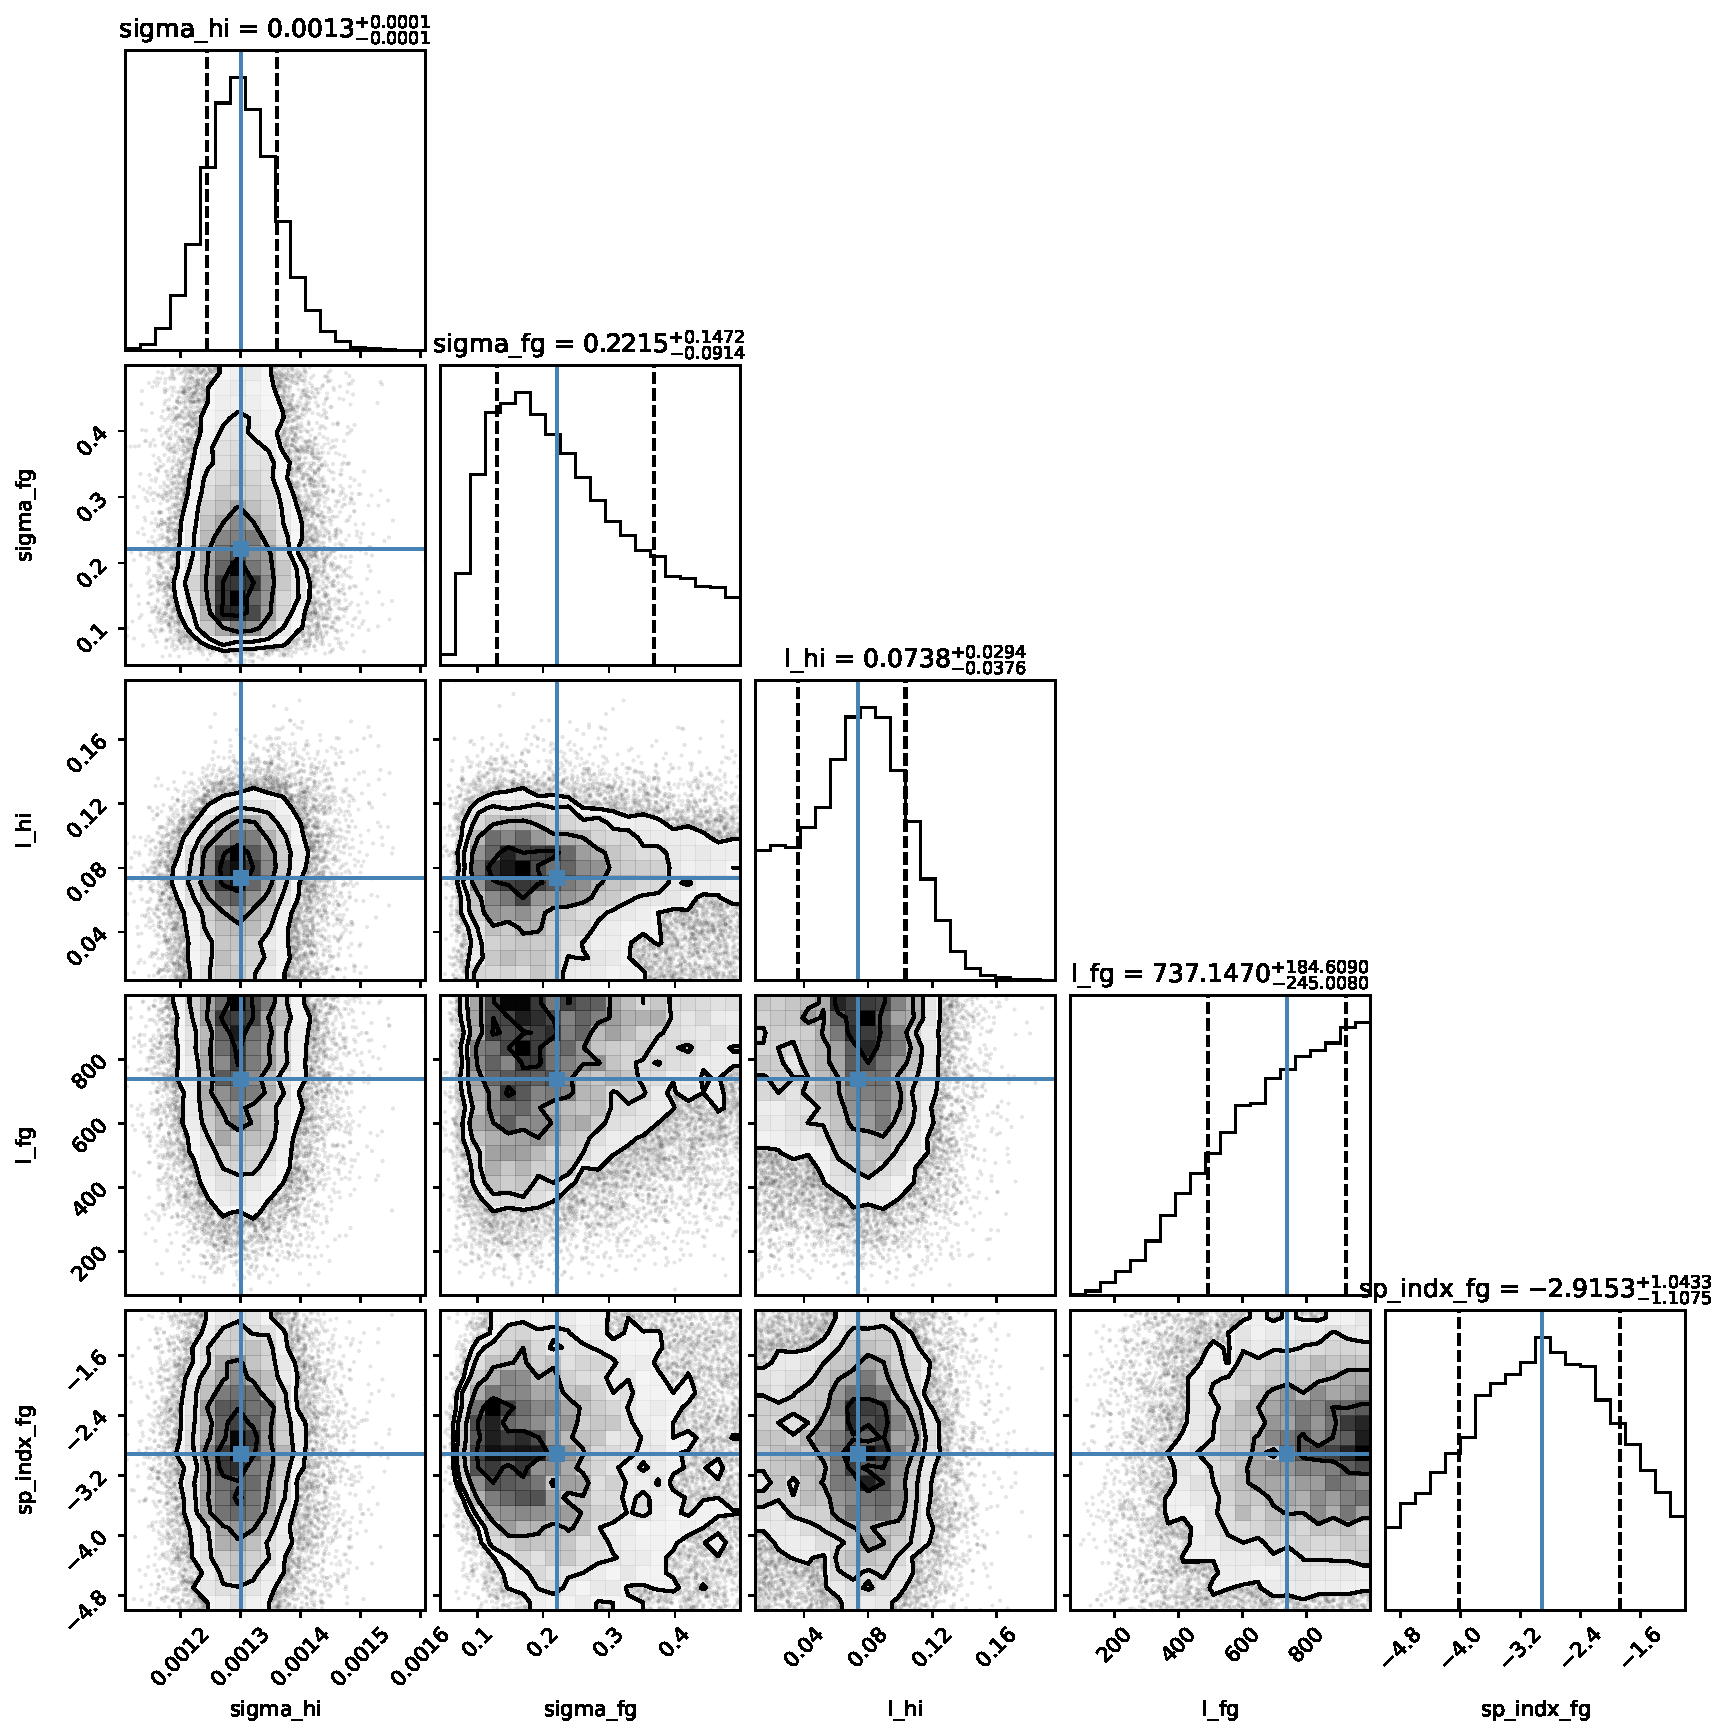
\includegraphics[width=1\linewidth]{outputs/week8/mcmc_corner_plot_with_sp_indx_fg_1.pdf}
    \caption{Enter Caption}
    \label{fig:placeholder}
\end{figure}

\clearpage

\begin{figure}[htb!]
    \centering
    \begin{minipage}{0.49\textwidth}
        \centering
        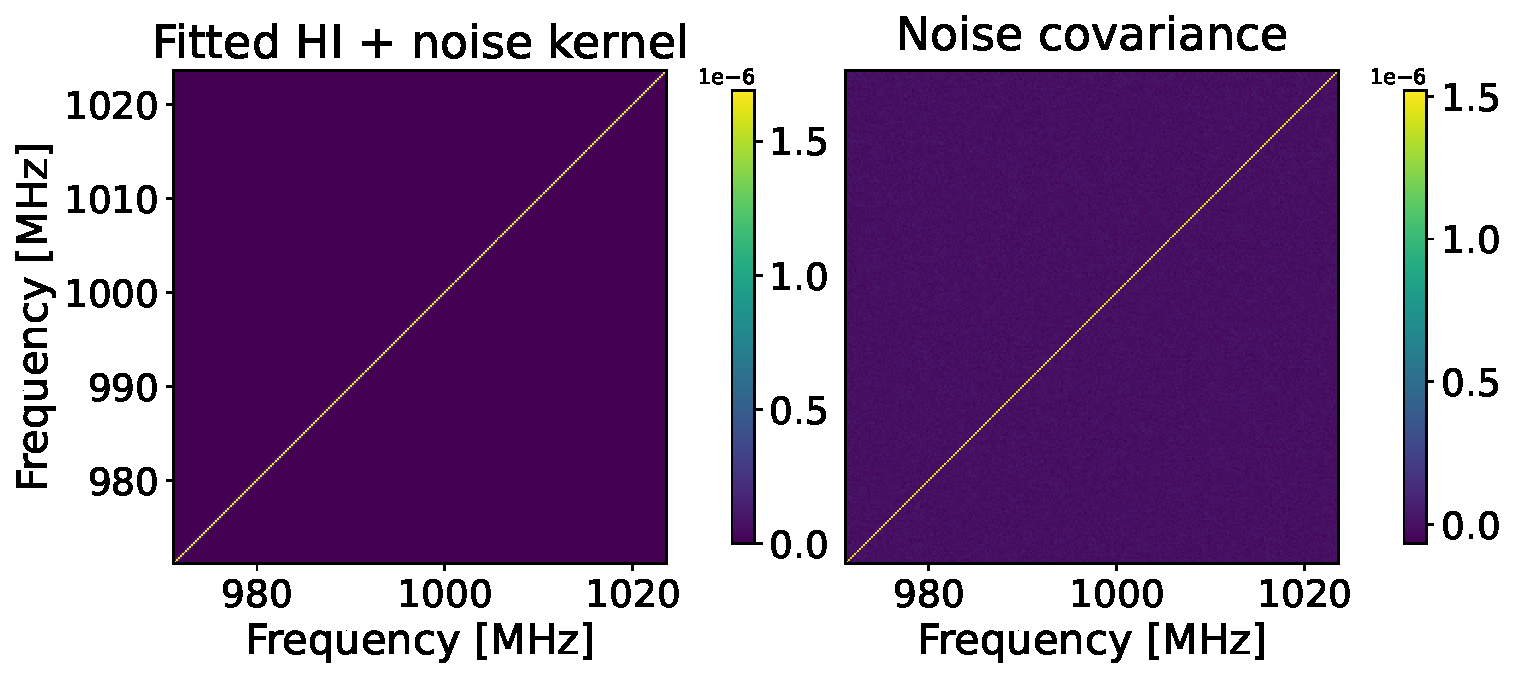
\includegraphics[width=\linewidth]{outputs/week8/hi_signal_kernal_comparison_mcmc_with_sp_indx_fg_1.pdf}
        \label{fig:pspec_lin_0_01}
    \end{minipage}
    \hfill
    \begin{minipage}{0.49\textwidth}
        \centering
        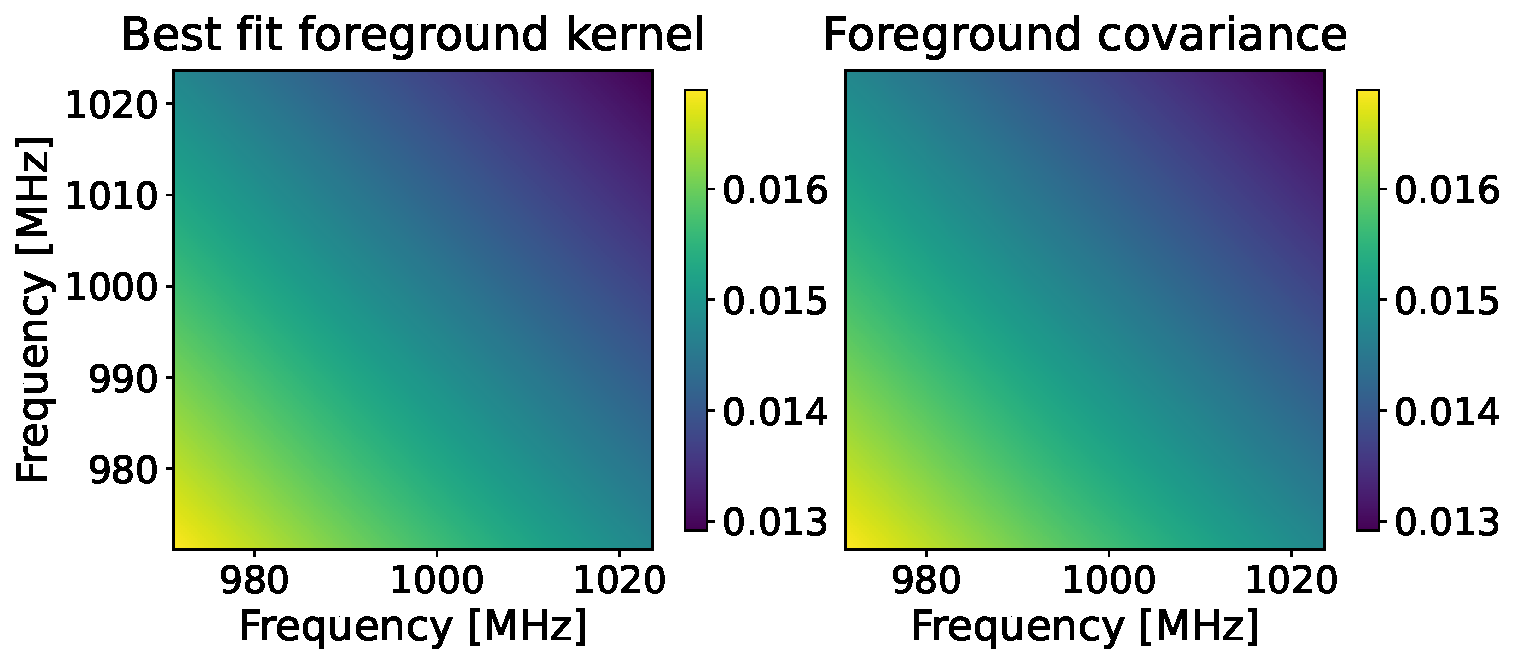
\includegraphics[width=\linewidth]{outputs/week8/fg_signal_kernal_comparison_mcmc_with_sp_indx_fg_1.pdf}
        \label{fig:pspec_log_0_01}
    \end{minipage}
    \caption{Enter Caption}
\end{figure}

\begin{figure}[hbt!]
    \centering
    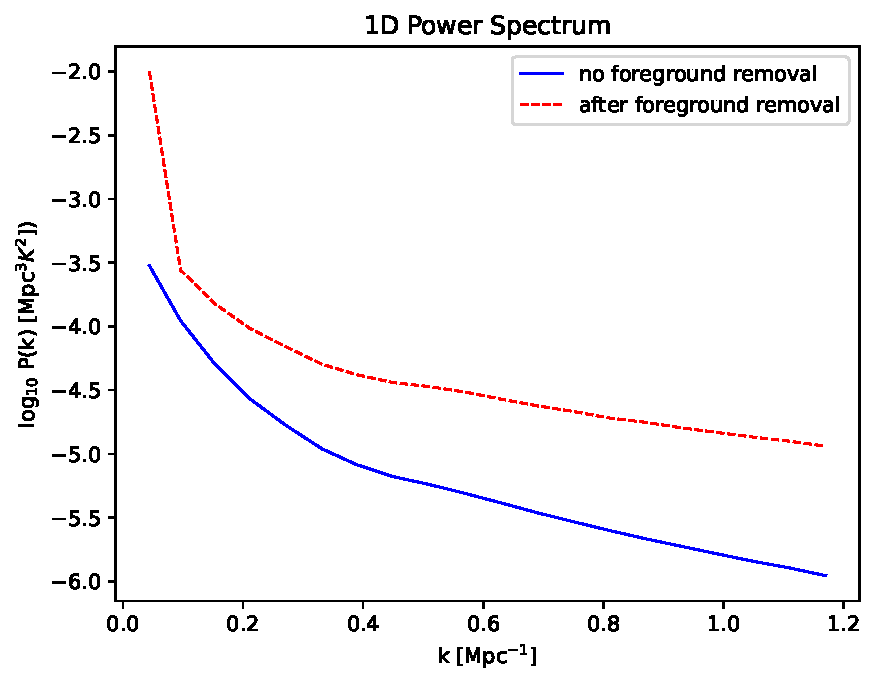
\includegraphics[width=0.4\linewidth]{outputs/week8/log_1d_power_spectrum_mcmc_with_sp_indx_fg_1.pdf}
    \caption{Enter Caption}
    \label{fig:placeholder}
\end{figure}

\begin{figure}[hbt!]
    \centering
    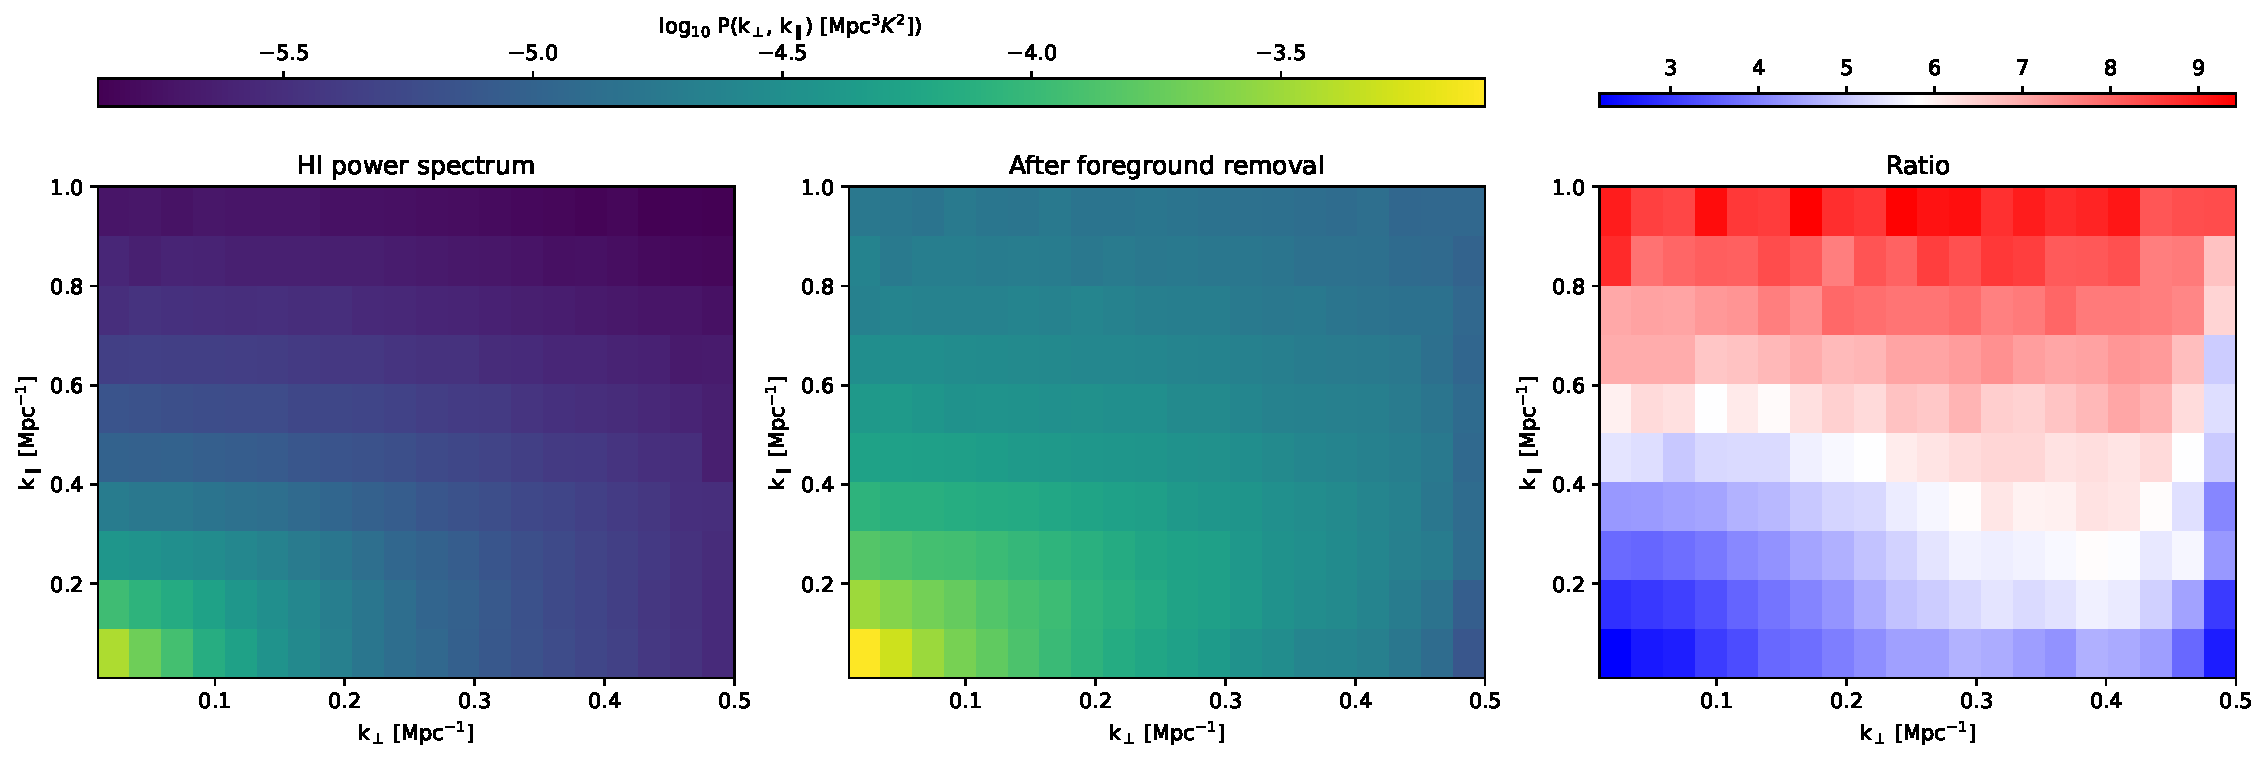
\includegraphics[width=0.9\linewidth]{outputs/week8/cylindrical_power_spectrum_mcmc_with_sp_indx_fg_1.pdf}
    \caption{Enter Caption}
    \label{fig:placeholder}
\end{figure}

\clearpage

\subsubsection{MCMC with spectral index}

\begin{figure}[hbt!]
    \centering
    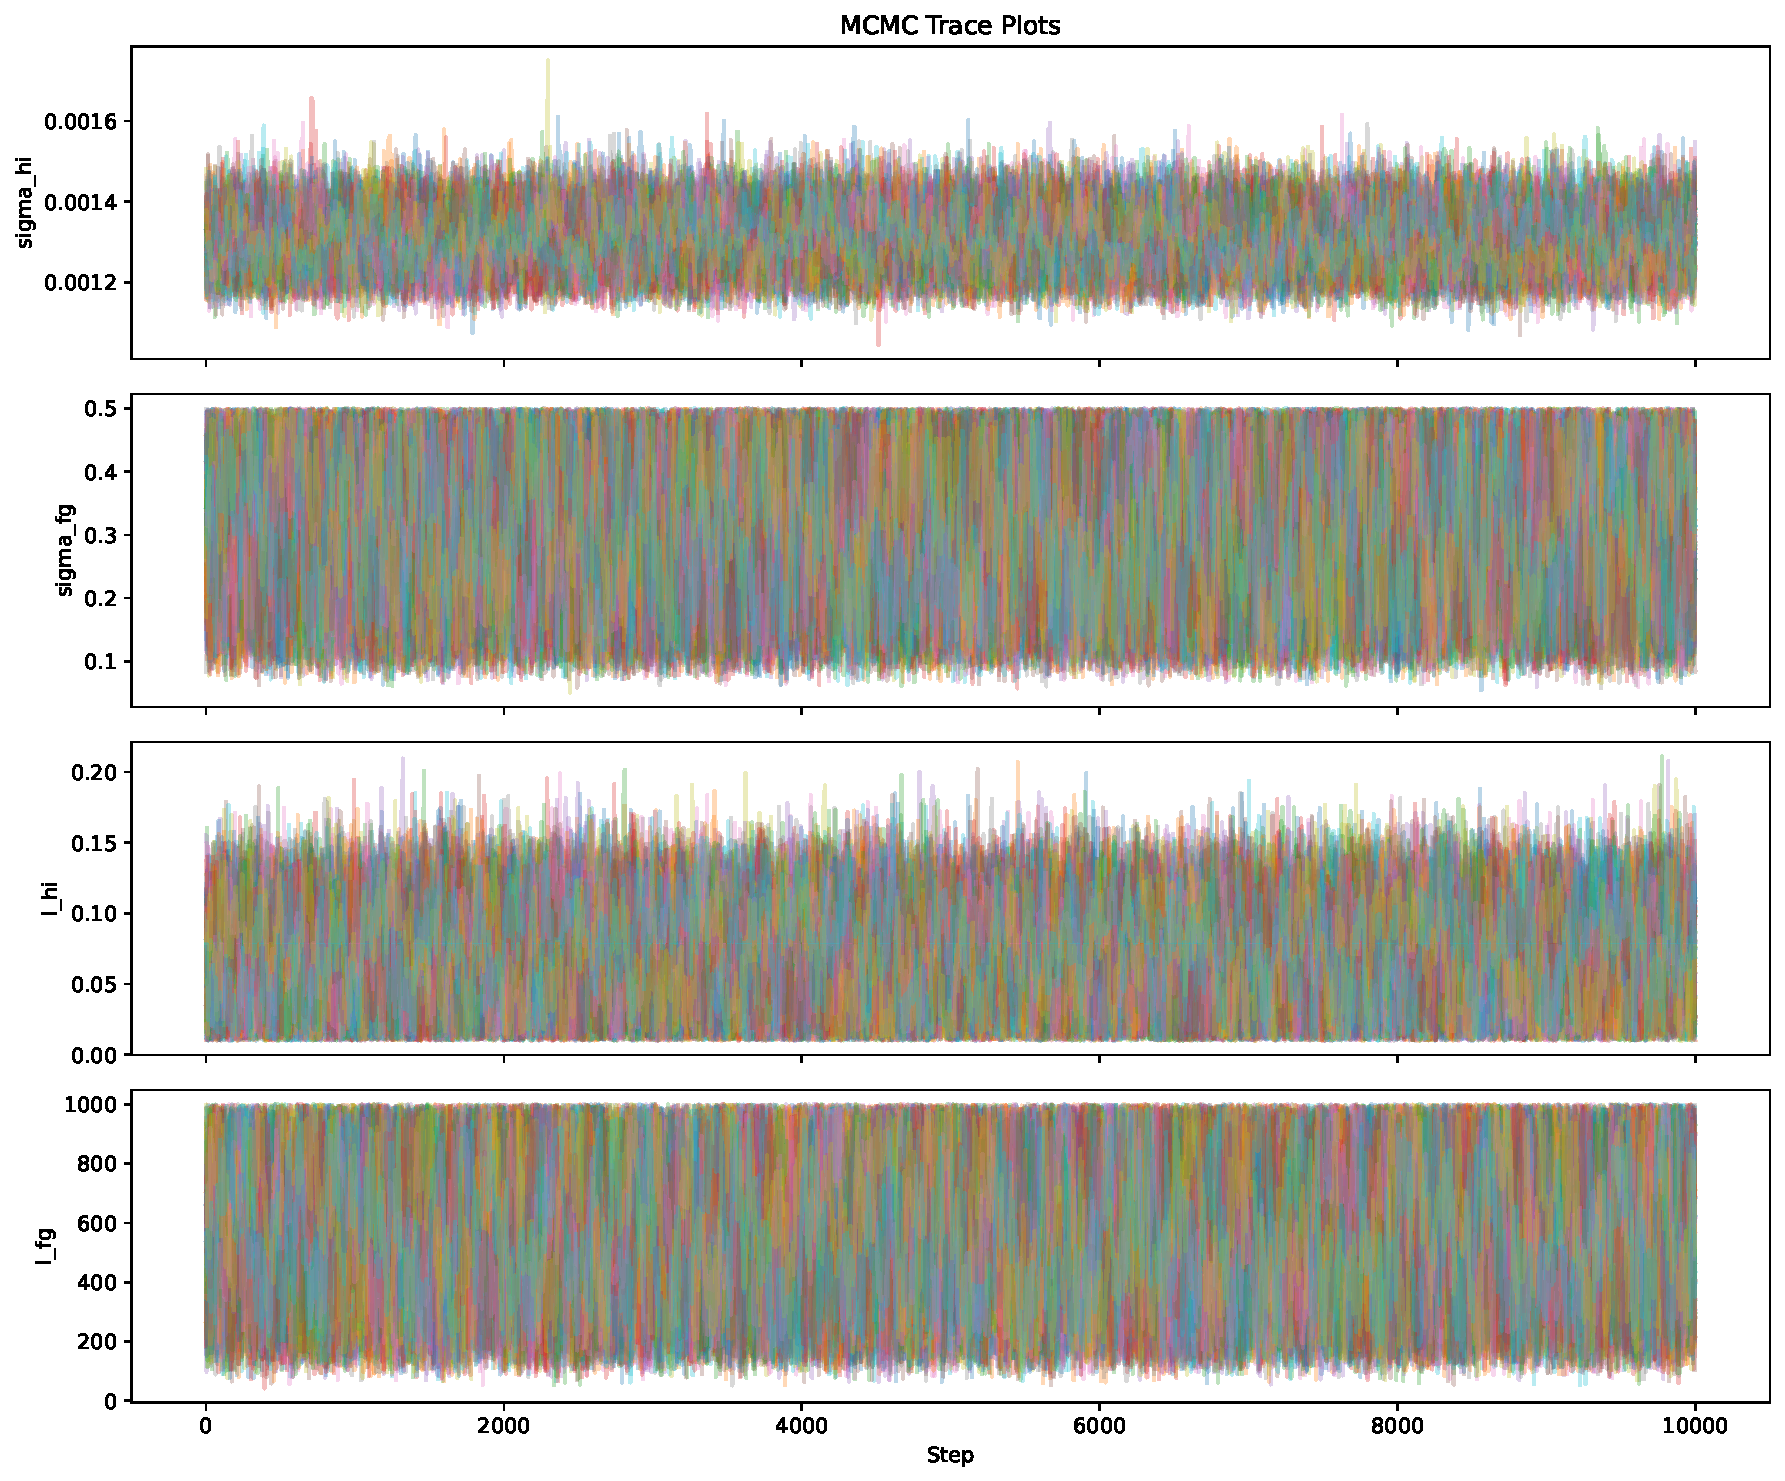
\includegraphics[width=1\linewidth]{outputs/week8/mcmc_chain_without_sp_indx_fg_2.pdf}
    \caption{Enter Caption}
    \label{fig:placeholder}
\end{figure}

\begin{figure}[hbt!]
    \centering
    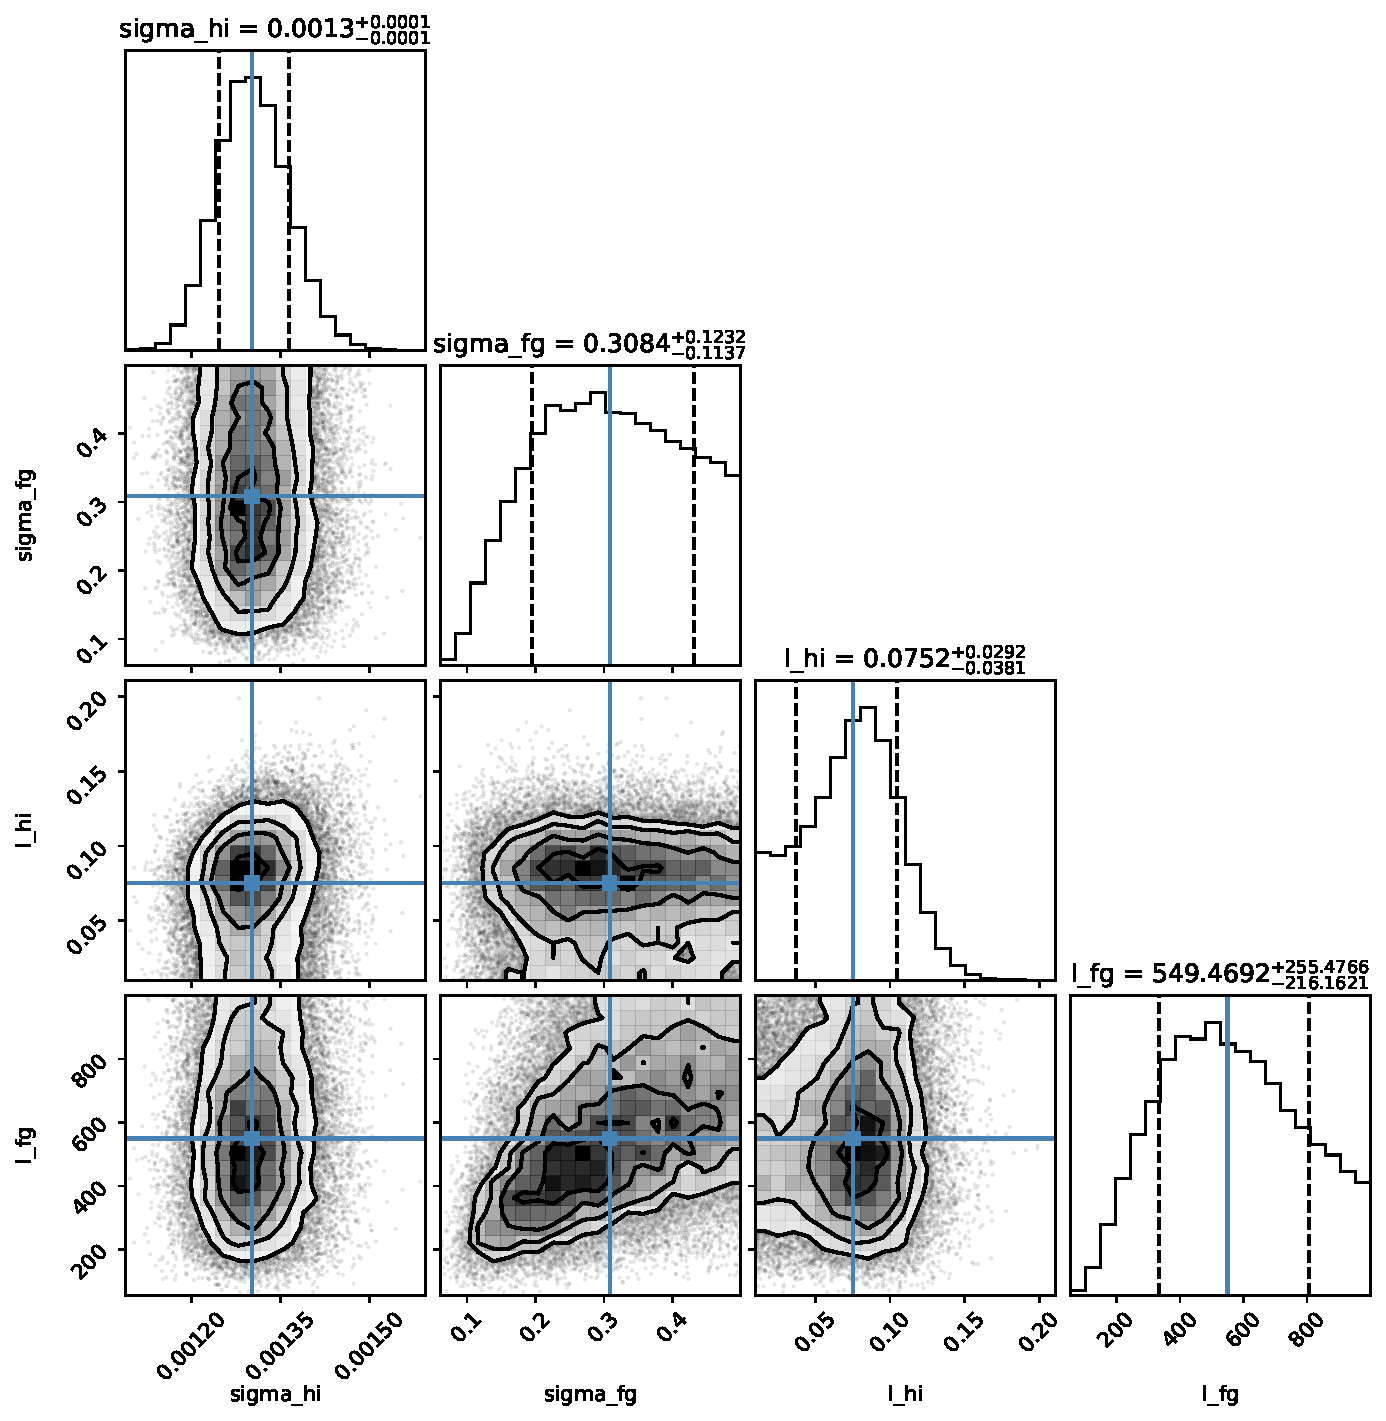
\includegraphics[width=1\linewidth]{outputs/week8/mcmc_corner_plot_without_sp_indx_fg_2.pdf}
    \caption{Enter Caption}
    \label{fig:placeholder}
\end{figure}

\clearpage

\begin{figure}[htb!]
    \centering
    \begin{minipage}{0.49\textwidth}
        \centering
        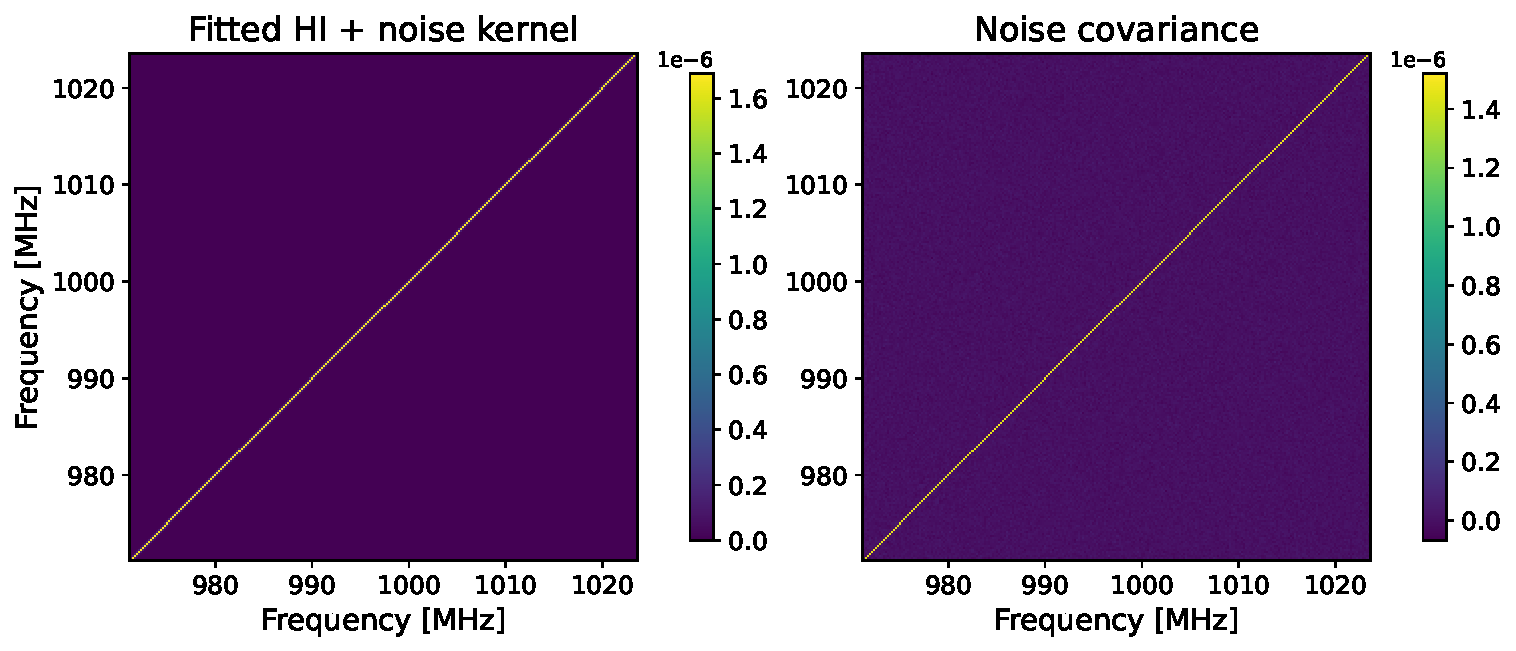
\includegraphics[width=\linewidth]{outputs/week8/hi_signal_kernal_comparison_mcmc_without_sp_indx_fg_2.pdf}
        \label{fig:pspec_lin_0_01}
    \end{minipage}
    \hfill
    \begin{minipage}{0.49\textwidth}
        \centering
        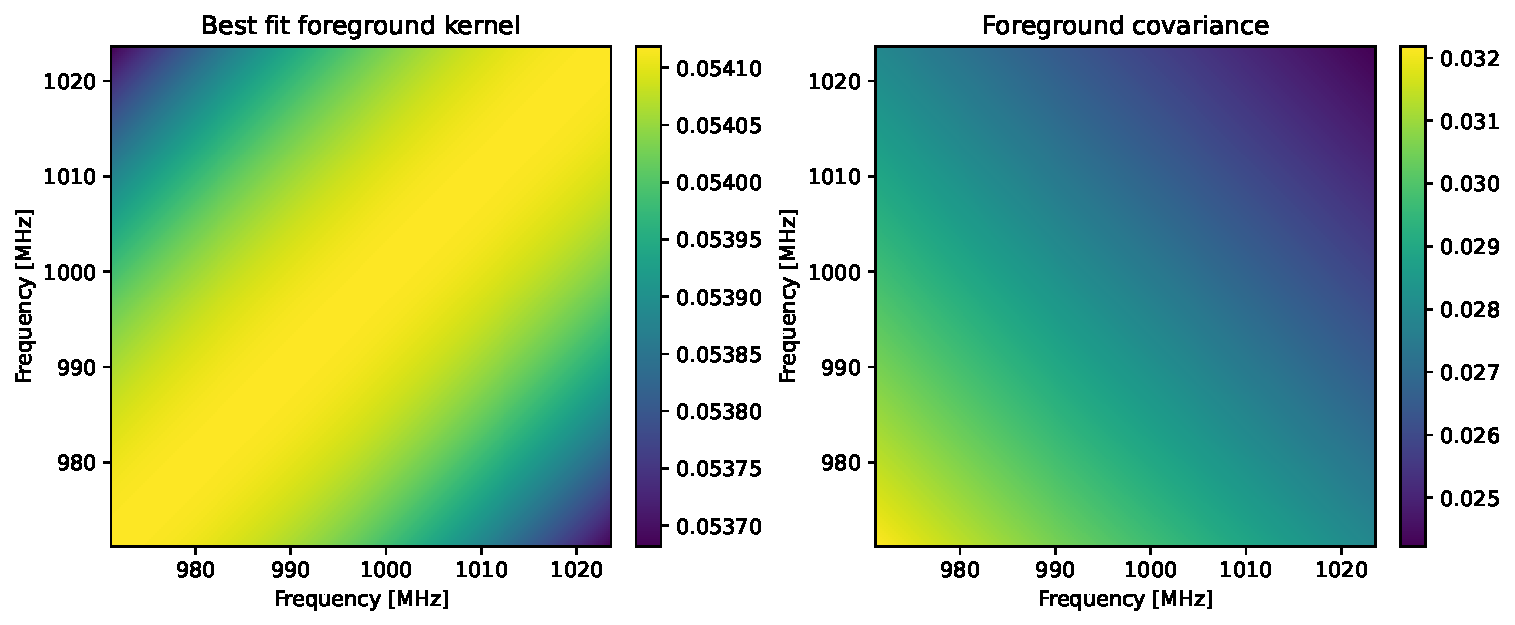
\includegraphics[width=\linewidth]{outputs/week8/fg_signal_kernal_comparison_mcmc_without_sp_indx_fg_2.pdf}
        \label{fig:pspec_log_0_01}
    \end{minipage}
    \caption{Enter Caption}
\end{figure}

\begin{figure}[hbt!]
    \centering
    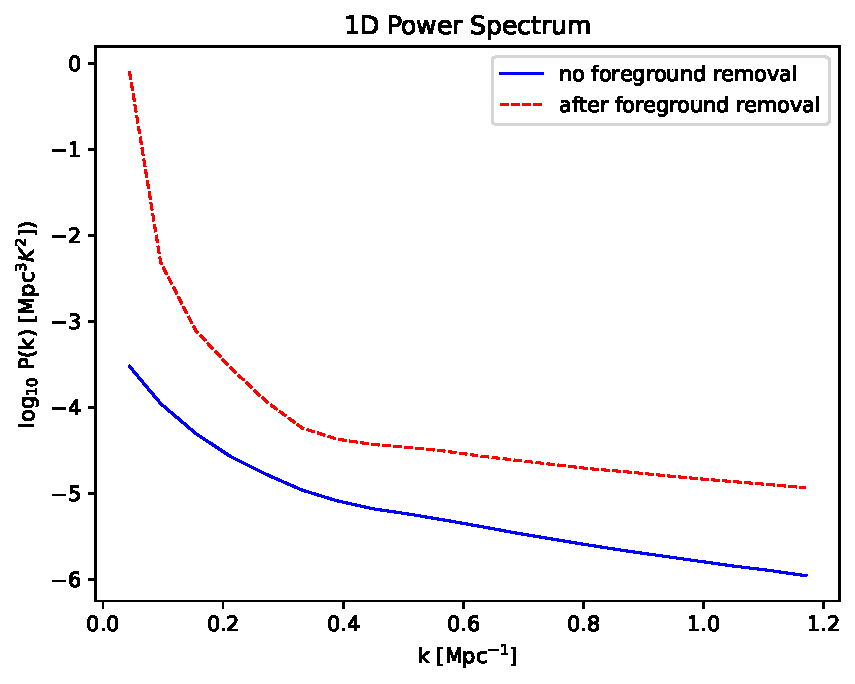
\includegraphics[width=0.4\linewidth]{outputs/week8/log_1d_power_spectrum_mcmc_without_sp_indx_fg_2.pdf}
    \caption{Enter Caption}
    \label{fig:placeholder}
\end{figure}

\begin{figure}[hbt!]
    \centering
    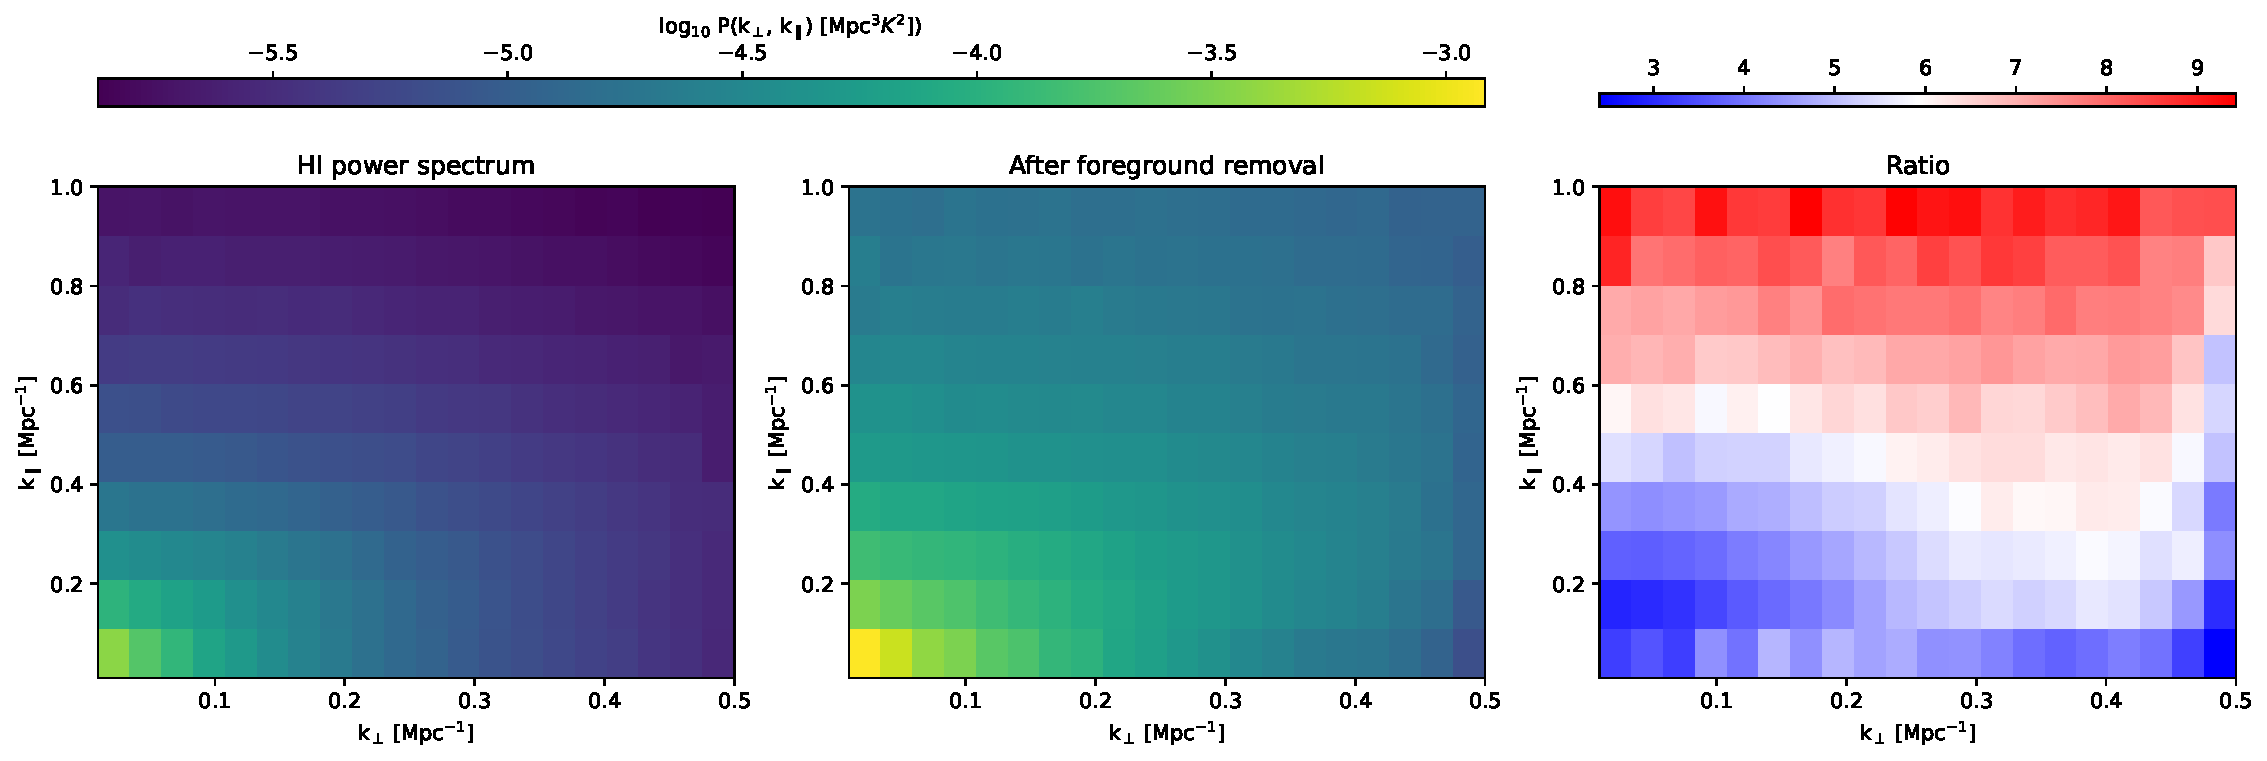
\includegraphics[width=0.9\linewidth]{outputs/week8/cylindrical_power_spectrum_mcmc_without_sp_indx_fg_2.pdf}
    \caption{Enter Caption}
    \label{fig:placeholder}
\end{figure}

\clearpage

\subsection{Wednesday 4th March}

Zhaoting sent an email with some feedback for my draft 5 page report. Here is a summary of the email:

\begin{itemize}
    \item Mainly the way I phrased some parts of my introduction, I should change to better match an academic paper and help gain the attention of my reader
        \item Some comments about figures such as making them look a bit nicer, having larger text sizes
        \item The cylindrical power spectrum should be run with 100 realisations
\end{itemize}

\subsection{Thursday 5th March}

\subsubsection{Meeting 7: Zhaoting}

\begin{itemize}
    \item Today, we primarily went over my draft report and his feedback.
    \item All of the feedback is written in the email but in the meeting more feedback was given:
\begin{itemize}
    \item I should combine my "Foreground removal techniques section" and "Methodology" section so it's just one coherent section. Do not split the theory then my methods for the code, just explain it as it goes. Makes more sense to the reader this way.
    \item For the PCA section, either go into more detail with the equations and the maths or remove the equations completely and just explain using my plots
\end{itemize}
\item In one of the papers, I read that PCA is expected to have signal loss at low k but my final graph shows the opposite of what is expected.
\begin{itemize}
    \item This is because I account for this when I set the lower bounds of k perp and k para to avoid this signal loss. Before doing this, there is obvious signal loss.
    \item Make sure to show this graph before putting in lower bounds for k perp and k para.
\end{itemize}
\item Make sure to also include graphs for my steps to getting to the final results and explain everything. Do not just include the final results.
\item I also expressed some concern with my results for GPR. I can't seem to get any optimisation routines working.
\begin{itemize}
    \item Zhaoting suggested trying different kernels instead. I will do that for the next meeting.
\end{itemize}
\item I also need to start working on my report. Need to make sure I put enough time into it as the report makes up the majority of my grade. Doesn't matter if my results are good if the report doesn't show that.
\end{itemize}